\chapter{Airborne position} \label{chap:airborn-position}

The aircraft airborne position message is used to broadcast the position and altitude of the aircraft. It has the Type Code from 9 to 18 or from 20 to 22. When Type Code is from 9 to 18, the encoded altitude represents the barometric altitude of the aircraft. When the Type Code is from 20 to 22, the encoded altitude contains the GNSS altitude of the aircraft. The Type Code value is related to the uncertainties in the position, which will be discussed in a later chapter.

The structure of the ADS-B airborne position message payload is shown as follows:

\begin{verbatim}
+-------+-------+--------+---------+------+------+-------------+-------------+
| TC, 5 | SS, 2 | SAF, 1 | ALT, 12 | T, 1 | F, 1 | LAT-CPR, 17 | LON-CPR, 17 |
+-------+-------+--------+---------+------+------+-------------+-------------+
\end{verbatim}

There are eight fields in the message payload, and the details of all fields are listed in Table \ref{tb:adsb-air-pos-fields}.

\begin{table}[ht]
\caption{Airborne position message structure}
\label{tb:adsb-air-pos-fields}
\begin{tabular}{|l|l|l|l|l|}
\hline
\textbf{FIELD} & \textbf{} & \textbf{MSG} & \textbf{MB} & \textbf{BITS} \\ \hline
\begin{tabular}[c]{@{}l@{}}Type Code\\ ~~9-18: with barometric altitude\\ ~~20-22: with GNSS altitude\end{tabular} & TC & 33-37 & 1-5 & 5 \\ \hline
\begin{tabular}[c]{@{}l@{}}Surveillance status\\ ~~0: No condition\\ ~~1: Permanent alert\\ ~~2: Temporary alert\\ ~~3: SPI condition\end{tabular} & SS & 38-39 & 6-7 & 2 \\ \hline
Single antenna flag & SAF & 40 & 8 & 1 \\ \hline
Encoded altitude & ALT & 41-52 & 9-20 & 12 \\ \hline
Time & T & 53 & 21 & 1 \\ \hline
\begin{tabular}[c]{@{}l@{}}CPR Format\\  ~~0: even frame\\  ~~1: odd frame\end{tabular} & F & 54 & 22 & 1 \\ \hline
Encoded latitude & LAR-CPR & 55-71 & 23-39 & 17 \\ \hline
Encoded longitude & LON-CPR & 72-88 & 40-56 & 17 \\ \hline
\end{tabular}
\end{table}

It is important to emphasize that the encoded latitude and longitude are not the actual latitude and longitude values. Instead, the position information is encoded in a Compact Position Reporting (CPR) format, which requires fewer bits to encode positions with higher resolution. Two types of position messages (identified by the odd and even frame flag) are broadcast alternately. There are two different ways to decode an airborne position based on these messages:

\begin{enumerate}
\item \textbf{Globally unambiguous position decoding}: Without a known position to start with, using both types of messages to decode the position.
\item \textbf{Locally unambiguous position decoding}: Knowing a reference position from previous sets of messages, using only one message for the decoding.
\end{enumerate}


The position information in ADS-B messages is encoded in a compact position reporting (CPR) format. The general idea behind CPR is to encode more coordinate decimals using fewer bits. The CPR offers a trade-off between global position ambiguity and local position accuracy.


\section{A over-simplified example}
First of all, we will use a simple example to explain the basic ideas behind the CPR position encoding. CPR divides 2D space into two different grids. Two message types are used to encode the positions with different grids.

In the following simple example, we want to encode position $(9, 7)$ in a $16\times16$ discrete world. Normally, this would require 4 bits each to encode the $x$ and $y$ coordinates, which is $(1001, 0111)$.

In the simple "CPR" algorithm, we first define two different grids. The even grid has a size of $4\times4$, while the odd grid has a size of $5\times5$. The is illustrated in Figure \ref{fig:cpr_simple_1}.


\begin{figure}[!ht]
  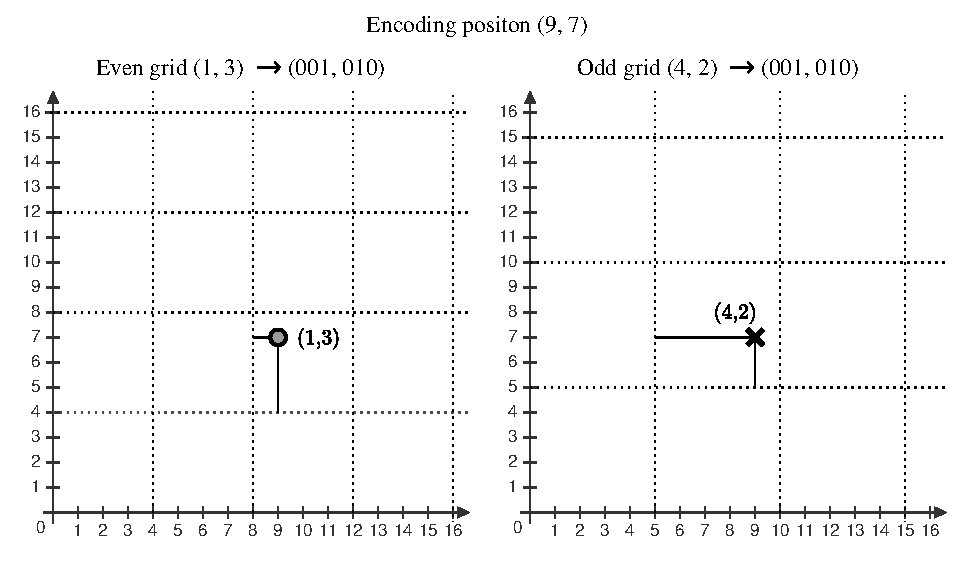
\includegraphics[width=0.9\linewidth]{figures/adsb/cpr_simple_1.pdf}
  \caption{Simplified CPR position coding (encoding)}
  \label{fig:cpr_simple_1}
\end{figure}

With these two grids, we can encode the local positions within each grid systems, which are $(1,3)$ and $(4,2)$ respectively. Now, the position can be encoded only using 3 bits. 

When the odd and even messages are received, each message alone has different possible global positions, which are shown in Figure \ref{fig:cpr_simple_2}.

\begin{figure}[!ht]
  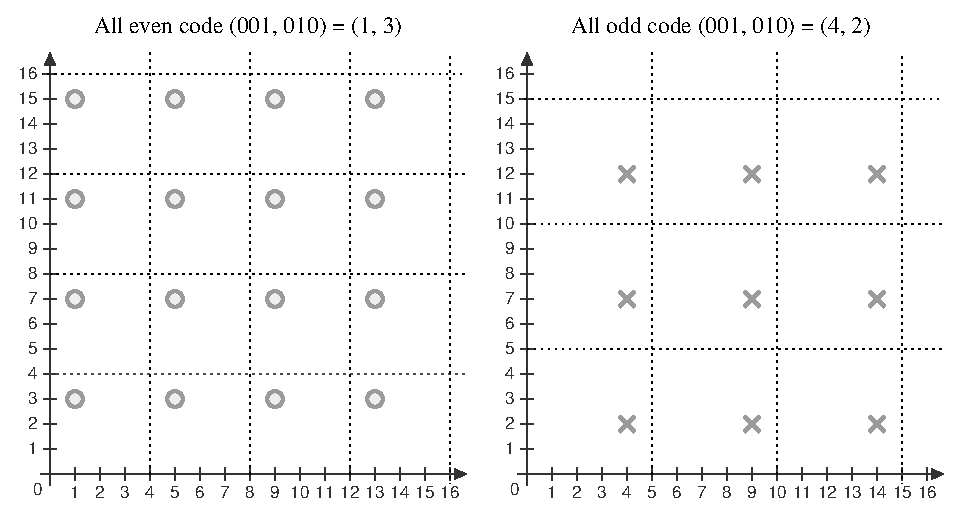
\includegraphics[width=0.9\linewidth]{figures/adsb/cpr_simple_2.pdf}
  \caption{Simplified CPR position coding (all position possiilities)}
  \label{fig:cpr_simple_2}
\end{figure}

Combining the possible positions from both even and odd messages, we can recover the global position where the solutions from both grids overlap with each other. This is shown in Figure \ref{fig:cpr_simple_3}.

\begin{figure}[!ht]
  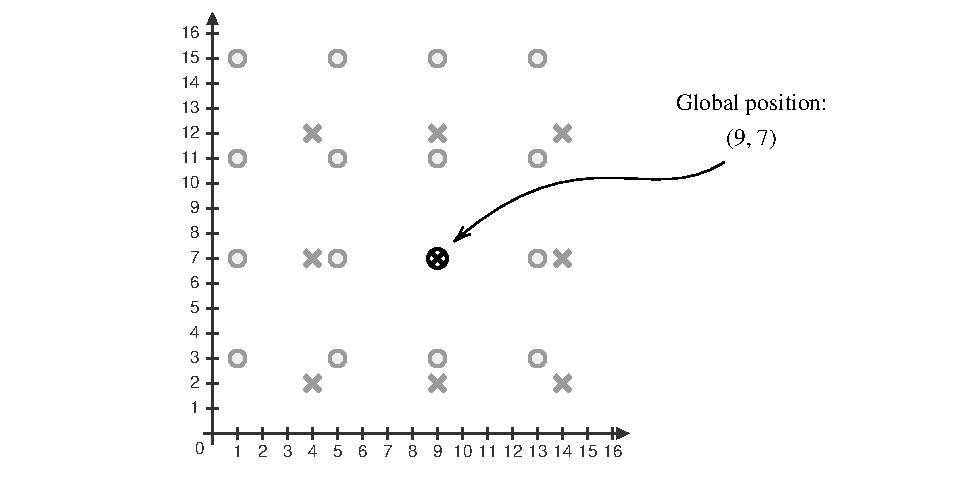
\includegraphics[width=0.9\linewidth]{figures/adsb/cpr_simple_3.pdf}
  \caption{Simplified CPR position coding (final global position)}
  \label{fig:cpr_simple_3}
\end{figure}

\newpage

\section{Compact position reporting}

\subsection{CPR zones}
The actual CPR algorithm is more sophisticated. First of all, more zones are defined. There are 15 latitude zones defined for each hemisphere. Up to 59 longitude zones are used, and the number of longitude zones is different at different altitudes.

In Figure \ref{fig:cpr_lat_zones}, the latitude zones are illustrated. The solid and dashed lines represent the latitude zone size of even and odd messages.

\begin{figure}
  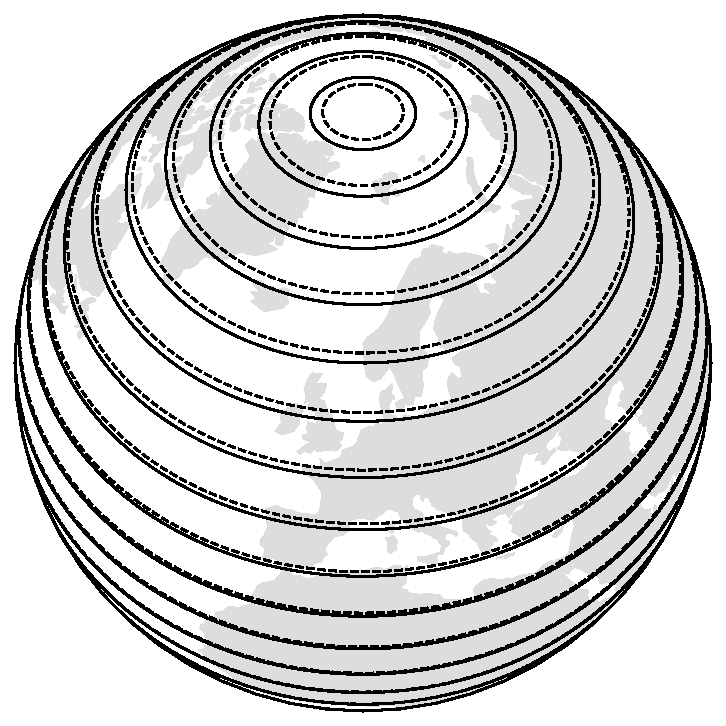
\includegraphics[width=0.7\linewidth]{figures/adsb/cpr_lat_zone_high.pdf} 
  \vspace{0.5cm}
  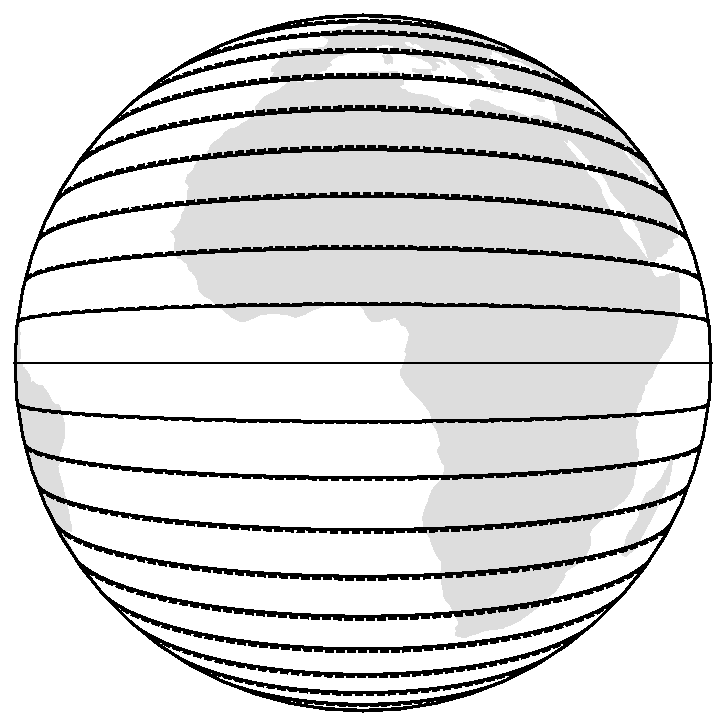
\includegraphics[width=0.7\linewidth]{figures/adsb/cpr_lat_zone_low.pdf}
  \caption{Latitude zones in compact position reporting, from different view points.}
  \label{fig:cpr_lat_zones}
\end{figure}

In Figure \ref{fig:cpr_lon_zones}, the latitude zones are illustrated. On the right-hand side of the figure is a zoomed-in view of the gird of northern Europe. The black and gray lines represent the longitude zone size of even and odd messages. We can see that the number of longitude zones (and the sizes) also differs depending on the latitude.

\begin{figure}
  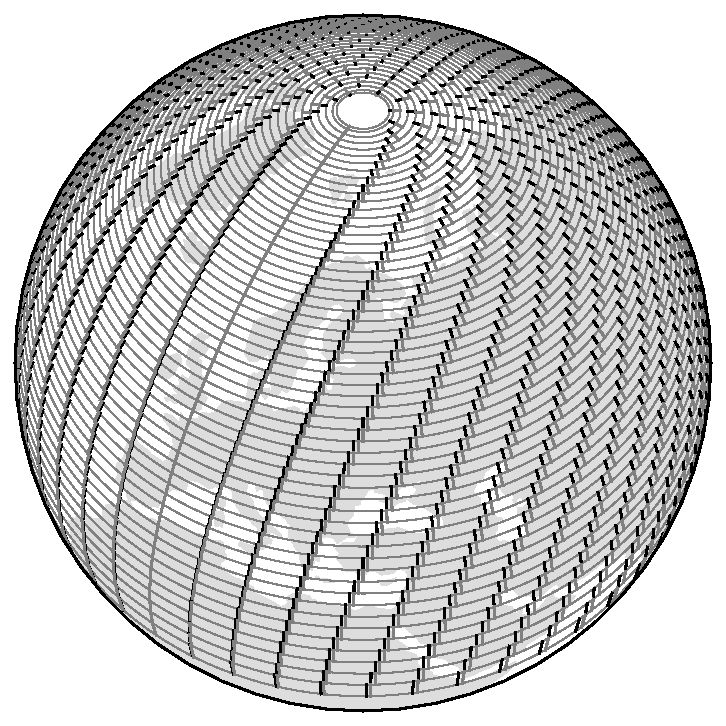
\includegraphics[width=0.7\linewidth]{figures/adsb/cpr_lon_zone_full.pdf}
  \vspace{0.5cm}
  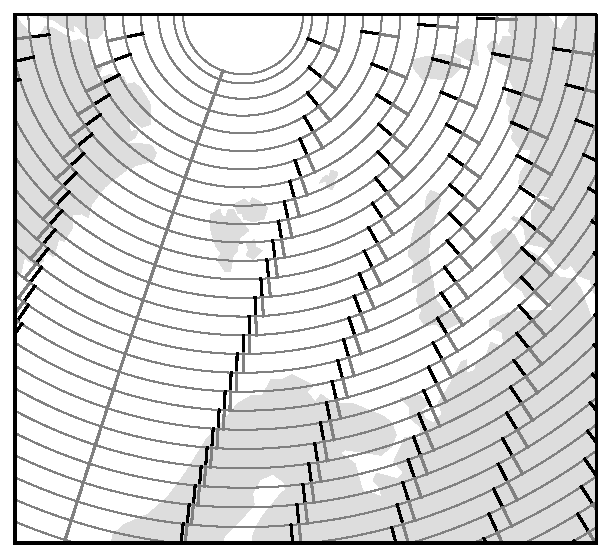
\includegraphics[width=0.7\linewidth]{figures/adsb/cpr_lon_zone_zoom.pdf}
  \caption{Longitude zones in position reporting}
  \label{fig:cpr_lon_zones}
\end{figure}

To report a position, the fractions of latitude and longitude in respective zones are encoded using 17 bits. These bits are transmitted in the position messages.


\subsection{Core functions and parameters}
To decode the CPR positions, we first introduce relevant parameters and common functions.

\subsubsection{Nz}

$N_Z$ represents the number of latitude zones between the equator and a pole. In Mode~S, $N_Z$ is defined to be 15.

\subsubsection{floor(x)}

The floor function $floor(x)$ returns the greatest integer value $k$, where $k \le x$. For example:

\begin{equation}
  \begin{split}
    floor(5.6) &= 5 \\
    floor(-5.6) &= -6
  \end{split}
\end{equation}

\subsubsection{mod(x, y)}

The modulo function is defined as:

\begin{equation}
  mod(x,y) = x - y \cdot floor \left( \frac{x}{y} \right), \qquad y \ne 0
\end{equation}

\subsubsection{NL(lat) - Longitude zone number}

Given the latitude, this function yields the number of longitude zones between 1 and 59. The function is expressed as:

\begin{equation}
  \mathrm{NL}(\mathrm{lat}) = floor \left\{ \dfrac{2 \pi}{\arccos \left[ 1 - \dfrac{1-\cos \left( \dfrac{\pi}{2~N_Z} \right)}{\cos^2\left(\dfrac{\pi}{180} \cdot \mathrm{lat} \right)} \right] } \right\}
\end{equation}

For latitudes that are close to the equator or the poles, one of following values is returned:

\begin{verbatim}
lat = 0     ->    NL = 59
lat = +87   ->    NL = 2
lat = -87   ->    NL = 2
lat > +87   ->    NL = 1
lat < -87   ->    NL = 1
\end{verbatim}


\section{Globally unambiguous position decoding} 

\subsection{Calculation of latitude} \label{sec:cpr_airborne_global_lat}

In each position message, bit 54 determines whether it is an odd or even type. \0 indicates an even message, while \1 indicates an odd message.

Bits 55-71 and bits 72-88 represent the fractions of the latitude and longitude within the latitude and longitude grid, denoted as $\mathrm{lat}_\mathrm{cpr}$ and $\mathrm{lon}_\mathrm{cpr}$:

\begin{equation}
  \begin{split}
      \mathrm{lat}_\mathrm{cpr} &= \frac{N_{cpr,lat}}{2^{17}} \\
    \mathrm{lon}_\mathrm{cpr} &= \frac{N_{cpr,lon}}{2^{17}}
  \end{split}
\end{equation}


For even and odd messages, the latitude zone sizes are defined as follows:

\begin{equation}
\begin{split}
  \mathrm{dLat}_\mathrm{even} &= \frac{360^\circ}{4 N_Z} \\
  \mathrm{dLat}_\mathrm{odd} &= \frac{360^\circ}{4 N_Z - 1}
\end{split}
\end{equation}


To decode the latitude, first, use the following equation to calculate the latitude zone index, demoted as $j$:

\begin{equation}
  j = floor \left( 59 \cdot \mathrm{lat}_\mathrm{cpr, even} - 60 \cdot \mathrm{lat}_\mathrm{cpr,odd} + \frac{1}{2}  \right)
\end{equation}


Based on both even and odd frames, two latitudes are computed as follows:

\begin{equation}
  \begin{split}
    \mathrm{lat}_\mathrm{even} &= \mathrm{dLat}_\mathrm{even} \Big( mod(j, 60) + \mathrm{lat}_\mathrm{cpr, even} \Big) \\
    \mathrm{lat}_\mathrm{odd} &= \mathrm{dLat}_\mathrm{odd} \Big( mod(j, 59) + \mathrm{lat}_\mathrm{cpr,odd} \Big)
  \end{split}
\end{equation}


For the southern hemisphere, values returned from previouse equations range from 270 to 360 degrees. Hence, we need to make sure the latitude is within the range of $[-90, +90]$ by applying the following equations:

\begin{equation}
  \begin{split}
    \mathrm{lat}_\mathrm{even} = \mathrm{lat}_\mathrm{even} - 360,  \quad &\text{if}~\mathrm{lat}_\mathrm{even} \ge 270 \\
    \mathrm{lat}_\mathrm{odd} = \mathrm{lat}_\mathrm{odd} - 360,  \quad &\text{if}~\mathrm{lat}_\mathrm{odd} \ge 270
  \end{split}
\end{equation}


Before proceeding to the longitude calculation, we need to compute $\mathrm{NL}(\mathrm{lat}_\mathrm{even})$ and $\mathrm{NL}(\mathrm{lat}_\mathrm{odd})$ to check if both values are the same. If not, this means the pair of messages are from different longitude zones, and it is not possible to compute the correct global position.

In this case, decoding should be stopped, and it is necessary to wait for a pair of messages that are from the same latitude zone. This situation happens when aircraft are flying across the boundaries of longitude zones.


The final latitude is chosen according to the time stamps of the messages as:

\begin{equation}
  \mathrm{lat} =
  \begin{cases}
   \mathrm{lat}_\mathrm{even}     & \text{if}~T_\mathrm{even} \ge T_\mathrm{odd} \\
   \mathrm{lat}_\mathrm{odd}     & \text{otherwise}
  \end{cases}
\end{equation}

where the current latitude is the more recent of these two latitudes.

\subsection{Calculation of longitude} \label{sec:cpr_airborne_global_lon}

First, the longitude index, $m$, can be calculated as:

\begin{equation}
  m = floor \left( \mathrm{lon}_\mathrm{cpr, even} \cdot \Big[ \mathrm{NL}(\mathrm{lat})-1 \Big] - \mathrm{lon}_\mathrm{cpr,odd} \cdot \mathrm{NL}(\mathrm{lat}) + \frac{1}{2}  \right)
\end{equation}


We also need to calculate the longitude zone size, which is dependent on the latitude. For even and odd messages, the number of longitude zones is defined as:

\begin{equation}
\begin{split}
  n_\mathrm{even} &= max[\mathrm{NL}(\mathrm{lat}), 1] \\
  n_\mathrm{odd} &= max[\mathrm{NL}(\mathrm{lat}-1), 1]
\end{split}
\end{equation}


The longitude zone sizes are defined as follows:

\begin{equation}
\begin{split}
  \mathrm{dLon}_\mathrm{even} &= \frac{360^\circ}{n_\mathrm{even}} \\
  \mathrm{dLon}_\mathrm{odd} &= \frac{360^\circ}{n_\mathrm{odd}}
\end{split}
\end{equation}


Then, the longitude is calculated as:

\begin{equation}
\begin{split}
  \mathrm{lon}_\mathrm{even} &= \mathrm{dLon}_\mathrm{even} \Big[ mod(m, n_\mathrm{even}) + \mathrm{lon}_\mathrm{cpr,even} \Big] \\
  \mathrm{lon}_\mathrm{odd} &= \mathrm{dLon}_\mathrm{odd} \Big[ mod(m, n_\mathrm{odd}) + \mathrm{lon}_\mathrm{cpr,odd} \Big]
  \end{split}
\end{equation}


Similarly, the final longitude is chosen according to the time stamps of the messages as:

\begin{equation}
  \mathrm{lon} =
  \begin{cases}
   \mathrm{lon}_\mathrm{even}     & \text{if}~T_\mathrm{even} \ge T_\mathrm{odd} \\
   \mathrm{lon}_\mathrm{odd}     & \text{otherwise}
  \end{cases}
\end{equation}


It is worth noting that the longitudes in position messages are between 0 and 360 degrees. We often need to convert them to the range between -180 and 180 degrees, which is consistent with aviation conventions. We can convert them as:

\begin{equation}
  \mathrm{lon} = \mathrm{lon} - 360,  \quad \text{if}~\mathrm{lon} \ge 180
\end{equation}

\subsection{Example}

The example contains two position messages that are received within 10 seconds. The first message is the most recent position message transmitted by the aircraft.

\begin{verbatim}
8D40621D58C382D690C8AC2863A7   (most recent)
8D40621D58C386435CC412692AD6
\end{verbatim}

Following the common ADS-B message structure, we can identify the ICAO address and payload as follows:

\begin{verbatim}
+----+--------+----------------+--------+
|    | ICAO   |      Data      |  PI    |
+----+--------+----------------+--------+
| 8D | 40621D | 58C382D690C8AC | 2863A7 |
| 8D | 40621D | 58C386435CC412 | 692AD6 |
+----+--------+----------------+--------+
\end{verbatim}

We can covert the message data into binary format:

\begin{verbatim}
+-------+-----+--------------+---+---+-------------------+-------------------+
| TC    |     | ALT          | T | F | CPR-LAT           | CPR-LON           |
+-------+-----+--------------+---+---+-------------------+-------------------+
| 01011 | 000 | 110000111000 | 0 | 0 | 10110101101001000 | 01100100010101100 |
| 01011 | 000 | 110000111000 | 0 | 1 | 10010000110101110 | 01100010000010010 |
+-------+-----+--------------+---+---+-------------------+-------------------+
\end{verbatim}

It is possible to extract the encoded CPR latitude and longitude binary and convert them to decimal format. Then, these values are divided by the $2^{17}$, representing the fractions of the positions within the latitude and longitude grids:

\begin{equation}
  \begin{split}
    \mathrm{lat}_\mathrm{cpr,even} &= \frac{93000}{2^{17}} \\
    \mathrm{lon}_\mathrm{cpr,even} &= \frac{51372}{2^{17}} \\
    \mathrm{lat}_\mathrm{cpr,odd} &=  \frac{74158}{2^{17}} \\
    \mathrm{lon}_\mathrm{cpr,odd} &=  \frac{50194}{2^{17}}
  \end{split}
\end{equation}

We can calculate the latitude index, $j$, as:

\begin{equation}
  j = floor \left( 59 \times \frac{93000}{2^{17}} - 60 \times \frac{51372}{2^{17}} + \frac{1}{2}  \right) = 8
\end{equation}

Then, we can decode the latitudes from both even and odd messages:

\begin{equation}
  \begin{split}
    \mathrm{lat}_\mathrm{even} &= \frac{360}{4 \times 15} \Big[ mod(8, 60) + \frac{93000}{2^{17}} \Big] = 52.25720214843750 \\
    \mathrm{lat}_\mathrm{odd} &= \frac{360}{4 \times 15 - 1} \Big[ mod(8, 59) + \frac{74158}{2^{17}} \Big] = 52.26578017412606
  \end{split}
\end{equation}

After validating the longitude zone of both messages:

\begin{equation}
  \begin{split}
    \mathrm{NL}(\mathrm{lat}_\mathrm{even}) &= \mathrm{NL}(52.25720214843750) = 36 \\
    \mathrm{NL}(\mathrm{lat}_\mathrm{odd}) &= \mathrm{NL}(52.26578017412606) = 36
  \end{split}
\end{equation}

we can continue to calculate the global position. Since the even message is the most recent message, the latitude is:

\begin{equation}
  \mathrm{lat} = \mathrm{lat}_\mathrm{even} = 52.25720214843750
\end{equation}

The final longitude (based on the even message) is calculated as:

\begin{align}
  m &= floor \left( \frac{51372}{2^{17}} \times (36-1) - \frac{50194}{2^{17}} \times 36 + \frac{1}{2}  \right) = 0\\
  n &= max \Big( 36-0, 1 \Big) = 36\\
    \mathrm{lon} &= \frac{360}{36} \Big[ mod(0, 36) + \frac{51372}{2^{17}} \Big] = 3.91937255859375
\end{align}

\begin{notebox}{Try it out}
Using \texttt{pyModeS}, we can perform the previous calculation of globally unambiguous position as: 

\begin{verbatim}
import pyModeS as pms

msg0 = "8D40621D58C382D690C8AC2863A7"
msg1 = "8D40621D58C386435CC412692AD6"
t0 = 1457996402
t1 = 1457996400

position = pms.adsb.position(msg0, msg1, t0, t1)
\end{verbatim}

\end{notebox}



\section{Locally unambiguous position decoding}

Previously, a globally unambiguous position has been decoded using a pair of odd and even messages. In this part, we will discuss how to decode the ADS-B position with one message and a previous reference position that is obtained using globally unambiguous decoding.

This method offers the possibility to continuous decode aircraft using only one message. It computes the latitude index (j) and the longitude index (m) based on this existing reference position and can be applied to both odd and even messages.

\subsection{The reference position}

The reference position should be close to the actual position, which must be within a 180 NM range. For example, this can be the position of aircraft that is decoded in the previous update. The range limitation is to ensure the consistency of the latitude and longitude zones between the reference position and decoding position. The reference position is denoted as ($\mathrm{lat}_\mathrm{ref}$, $\mathrm{lon}_\mathrm{ref}$).

\subsection{Calculation of latitude}

Denote $i$ as the value dependent on the type of the message:

\begin{equation}
  i =
  \begin{dcases}
    0, \quad \text{even message} \\
    1, \quad \text{odd message}
  \end{dcases}
\end{equation}

\noindent The latitude zone size is different depending on the message type:

\begin{equation}
  \mathrm{dLat} = \frac{360}{4n_z-i}
\end{equation}

Then, the latitude zone index, $j$, is calculated as:

\begin{equation}
  j = floor \left( \frac{\mathrm{lat}_\mathrm{ref}}{\mathrm{dLat}} \right) + floor \left[ \frac{mod(\mathrm{lat}_\mathrm{ref}, \mathrm{dLat})}{\mathrm{dLat}}  - \mathrm{lat}_\mathrm{cpr}  + \frac{1}{2} \right]
\end{equation}

Knowing the latitude zone index, the latitude of the new position is:

\begin{equation}
  \mathrm{lat} = \mathrm{dLat} \cdot (j + \mathrm{lat}_\mathrm{cpr})
\end{equation}


\subsection{Calculation of longitude}

Next, we can calculate the increment of the longitude per zone based on the decoded latitude, which is dependent on both message type and latitude:

\begin{equation}
  \mathrm{dLon} = \frac{360}{max\Big( \mathrm{NL}(\mathrm{lat})-i, 1 \Big)}
\end{equation}


Then, the longitude zone index, $m$, is calculated as:

\begin{equation}
  m = floor \left( \frac{\mathrm{lon}_\mathrm{ref}}{\mathrm{dLon}} \right) + floor \left( \frac{mod(\mathrm{lon}_\mathrm{ref}, \mathrm{dLon})}{\mathrm{dLon}}  - \mathrm{lon}_\mathrm{cpr}  + \frac{1}{2}  \right)
\end{equation}

Knowing the longitude zone index, the longitude of the new position is:

\begin{equation}
  \mathrm{lon} = \mathrm{dLon} \cdot (m + \mathrm{lon}_\mathrm{cpr})
\end{equation}


\subsection{Example}

Next, we illustrate the decoding process of the messages from the previous example with a reference position. The message and the reference position are as follows:

\begin{verbatim}
Message: 8D40621D58C382D690C8AC2863A7
Data:            58C382D690C8AC

Reference position: (52.258, 3.918)
\end{verbatim}

We can easily covert the message data to binary:

\begin{verbatim}
+-------+-----+--------------+-----------------------------------------------+
| TC    |     | ALT          | T | F | CPR-LAT           | CPR-LON           |
|-------+-----+--------------+---+---+-------------------+-------------------|
| 01011 | 000 | 110000111000 | 0 | 0 | 10110101101001000 | 01100100010101100 |
+-------+-----+--------------+---+---+-------------------+-------------------+
|       |     |              |   |   | 93000             | 51372             |
+-------+-----+--------------+---+---+-------------------+-------------------+
\end{verbatim}

First, since this is an even message ($i=0$), we can calculate the latitude as follows:

\begin{align}
  \mathrm{dLat} &= \frac{360}{4 \times 15 - 0} = 6 \\
  j &= floor \left( \frac{52.258}{6} \right) + floor \left[ \frac{mod(52.258, 6)}{6} - \frac{93000}{2^{17}}  + \frac{1}{2} \right] = 8 \\
  \mathrm{lat} &= 6 \times \left( 8 + \frac{93000}{2^{17}} \right) = 52.2572021484375
\end{align}

Next, the longitude can be calculated as follows:

\begin{align}
  \mathrm{dLon} &= \frac{360}{max \Big( \mathrm{NL}(\mathrm{lat}_\mathrm{even})-0, 1 \Big)} = \frac{360}{max(36, 1)} = 10 \\
  m &= floor \left( \frac{3.918}{10} \right) + floor \left( \frac{mod(3.918, 10)}{10} - \frac{51372}{2^{17}}  + \frac{1}{2}  \right) = 0 \\
  \mathrm{lon} &= 10 \times \left(0 + \frac{51372}{2^{17}} \right) = 3.91937255859375
\end{align}

%
% d_lat:  6
% j:      8
% lat:    52.25720
% m:      0
% d_lon:  10
% lon:    3.91937

\begin{notebox}{Try it out}
Using \texttt{pyModeS}, we can perform the previous locally unambiguous position calculation as: 

\begin{verbatim}
import pyModeS as pms

msg = "8D40621D58C382D690C8AC2863A7"
lat_ref = 52.258
lon_ref = 3.918

position = pms.adsb.position_with_ref(msg, lat_ref, lon_ref)
\end{verbatim}

\end{notebox}


\section{Altitude decoding}

The altitude of the aircraft can be decoded with one position message, regardless of it being an even or odd type. However, depending on the type code of the messages, the altitudes are decoded differently. In Table \ref{tb:adsb-tc} from chapter \ref{chap:adsb-basic}, two different types of altitudes are shown. They are:

\begin{itemize}
\item \textbf{TC=9-18}: Airborne position, with barometric altitude encoded (in feet)
\item \textbf{TC=20-22}: Airborne position, with GNSS Height encoded (in meters)
\end{itemize}

\subsection{Barometric altitude}
For barometric altitude (TC between 9 and 18), the 8th bit of the 12-bit altitude field is the \emph{Q bit}. It indicates whether the altitude is encoded with an increment of 25 ft or 100 ft.

When $Q=1$, the altitude is encoded with a 25 ft increment. Removing the Q-bit, the altitude shall be the multiple of 25 ft minus 1000 ft:

\begin{equation}
  h = 25 ~ N - 1000 \quad \text{(ft)}
\end{equation}

For example, based the example message in the previous section, the 12 bits in the altitude field can be read as follows:

\begin{verbatim}
1100001 1 1000
        ^
       Q-bit
\end{verbatim}

Once the Q-bit is removed, the decimal representation of the remaining bits is 1560:

\begin{verbatim}
11000011000 -> 1560
\end{verbatim}

The altitude of the aircraft becomes:

\begin{equation}
1560 \times 25 - 1000 = 38000 \quad \text{(ft)}
\end{equation}

In the case where the altitude is higher than 50175 ft, a 100 ft increment is used. In this situation, the Q bit is set to \0, and the rest of the bits are encoded using Gray code.

It is worth noting that when all bits of the altitude fields are zeros, the altitude information is not available or not valid.


\subsection{GNSS height}

When the position message has the Type Code from 20 to 22, the 12-bit altitude field is used for the encoding of the GNSS height. The GNSS height is derived from the global positioning satellites, and the decimal value of all 12 bits translates into the height of aircraft in meters.

\begin{notebox}{Try it out}
Using \texttt{pyModeS}, we can perform the altitude decoding as: 

\begin{verbatim}
import pyModeS as pms

msg = "8D40621D58C382D690C8AC2863A7"

altitude = pms.adsb.altitude(msg)
\end{verbatim}

\end{notebox}



\section{Verification of decoded positions}

It is recommended to perform a \emph{reasonable test} to validate the decoded position. There are a couple of ways to perform such a reasonable test:

\begin{enumerate}
  \item The first approach is to use the receiver position. The decoded position should not exceed the coverage of the receiver. See chapter \ref{chap:quickstart}, Figure \ref{fig:max_range_curve}.

  \item A further test is to use more than one pair of different messages to produce multiple globally unambiguous positions. Then, the distance between these positions can be used to examine whether the decoded positions are reasonable.
\end{enumerate}

If the decoded position fails the reasonable tests, it should be discarded.
